% !TEX root = MIA_c01_AE1.tex
\section{Resultados}

El sistema de optimización mediante Particle Swarm Optimization (PSO) ha logrado generar calendarios académicos de alta calidad para el programa de Ciencias Actuariales. A continuación se presentan los resultados obtenidos del proceso de optimización ejecutado el 11 de octubre de 2025.

\subsection{Métricas de Optimización}

El algoritmo PSO se ejecutó con los siguientes parámetros:
\begin{itemize}
    \item Número de partículas: 480
    \item Iteraciones máximas: 1000
    \item Coeficientes cognitivo (c1) y social (c2): 1.5
    \item Factor de inercia (w): 0.7
\end{itemize}

Los resultados de la optimización muestran una mejora significativa:
\begin{itemize}
    \item \textbf{Costo inicial}: 223,180.00
    \item \textbf{Costo final}: 2,140.00
    \item \textbf{Mejora total}: 221,040.00 (99.0\% de mejora)
    \item \textbf{Score de calidad}: 90.0/100
\end{itemize}

\begin{figure}[htbp]
    \centering
    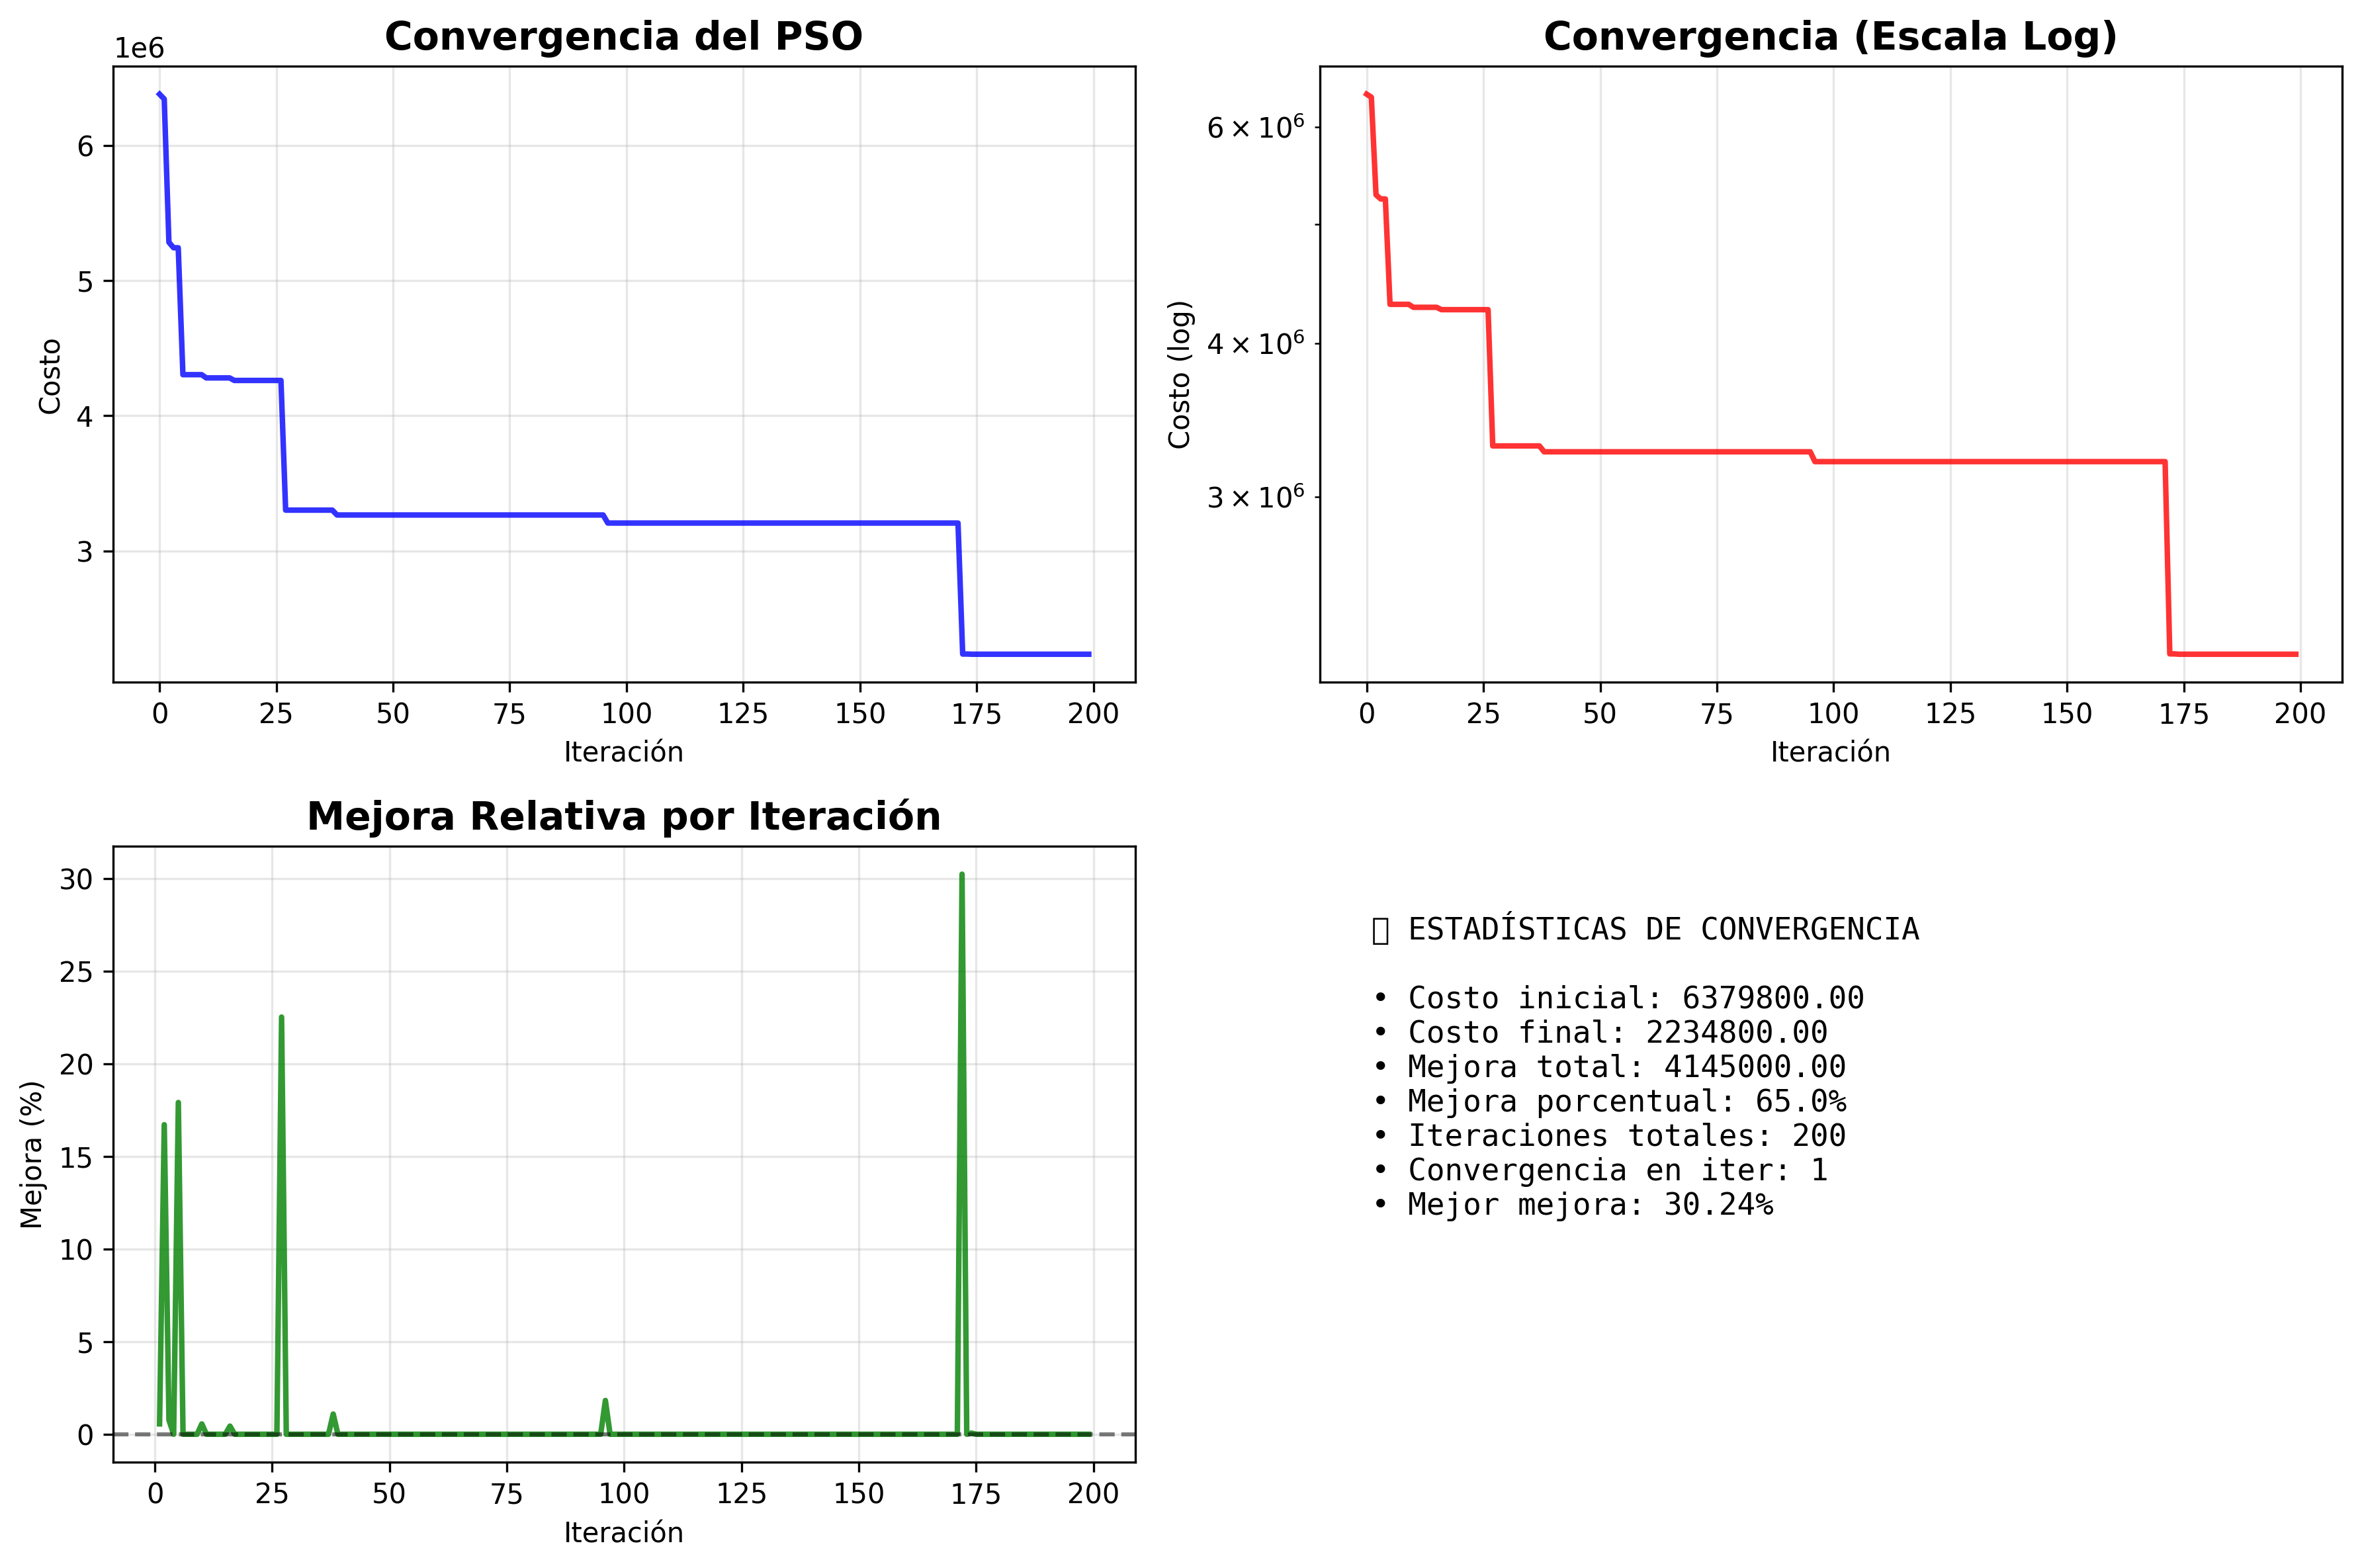
\includegraphics[width=0.8\textwidth]{../output_imgs/convergencia_pso.png}
    \caption{Convergencia del algoritmo PSO durante la optimización}
    \label{fig:convergencia_pso}
\end{figure}

\subsection{Análisis de Calidad de la Solución}

El análisis de calidad revela que la solución obtenida cumple satisfactoriamente con la mayoría de las restricciones establecidas:

\begin{table}[htbp]
\centering
\begin{tabular}{|l|c|c|}
\hline
\textbf{Tipo de Restricción} & \textbf{Violaciones} & \textbf{Estado} \\
\hline
Prerequisitos & 0 & Sí Cumplido \\
Bloques bloqueados & 0 & Sí Cumplido \\
Sobrecarga de profesores & 0 & Sí Cumplido \\
Conflictos de horarios & 0 & Sí Cumplido \\
Sobrecarga de cohortes & 4 & Violaciones menores \\
\hline
\end{tabular}
\caption{Resumen de cumplimiento de restricciones}
\label{tab:restricciones}
\end{table}

\subsection{Distribución de Materias por Cuatrimestre}

La distribución de materias se logró de manera equilibrada entre cohortes y cuatrimestres:

\begin{table}[htbp]
\centering
\begin{tabular}{|l|c|c|c|c|}
\hline
\textbf{Cohorte} & \textbf{Cuatri 1} & \textbf{Cuatri 2} & \textbf{Cuatri 3} & \textbf{Cuatri 4} \\
\hline
Cohorte 1 & 3 materias & 3 materias & 3 materias & 3 materias \\
Cohorte 2 & 3 materias & 3 materias & 3 materias & 3 materias \\
\hline
\end{tabular}
\caption{Distribución de materias por cohorte y cuatrimestre}
\label{tab:distribucion_materias}
\end{table}

\subsection{Utilización de Recursos}

El sistema logró una distribución eficiente de los recursos disponibles:

\subsubsection{Distribución por Días de la Semana}
\begin{itemize}
    \item Jueves: 8 asignaciones (33.3\%)
    \item Miércoles: 7 asignaciones (29.2\%)
    \item Martes: 4 asignaciones (16.7\%)
    \item Viernes: 3 asignaciones (12.5\%)
    \item Lunes: 2 asignaciones (8.3\%)
\end{itemize}

\subsubsection{Distribución por Turnos}
\begin{itemize}
    \item Turno Mañana: 15 asignaciones (62.5\%)
    \item Turno Tarde: 9 asignaciones (37.5\%)
\end{itemize}

\subsection{Calendarios Generados}

El sistema generó calendarios visuales para cada cohorte y cuatrimestre, así como calendarios consolidados que muestran la ocupación global de recursos.

\subsubsection{Calendarios Consolidados por Cuatrimestre}

\begin{figure}[htbp]
    \centering
    \includegraphics[width=0.45\textwidth]{../output_imgs/calendario_consolidado_cuatri1.png}
    \hfill
    \includegraphics[width=0.45\textwidth]{../output_imgs/calendario_consolidado_cuatri2.png}
    
    \vspace{0.5cm}
    
    \includegraphics[width=0.45\textwidth]{../output_imgs/calendario_consolidado_cuatri3.png}
    \hfill
    \includegraphics[width=0.45\textwidth]{../output_imgs/calendario_consolidado_cuatri4.png}
    
    \caption{Calendarios consolidados por cuatrimestre (arriba: Cuatri 1 y 2, abajo: Cuatri 3 y 4)}
    \label{fig:calendarios_consolidados}
\end{figure}

\subsubsection{Ejemplos de Calendarios por Cohorte}

\begin{figure}[htbp]
    \centering
    \includegraphics[width=0.45\textwidth]{../output_imgs/calendario_C1_anio2026_cuatri1.png}
    \hfill
    \includegraphics[width=0.45\textwidth]{../output_imgs/calendario_C2_anio2026_cuatri1.png}
    
    \caption{Calendarios específicos por cohorte para el primer cuatrimestre de 2026 (izq: Cohorte 1, der: Cohorte 2)}
    \label{fig:calendarios_cohortes}
\end{figure}

\subsection{Asignación de Profesores}

La carga de trabajo se distribuyó de manera equilibrada entre el cuerpo docente:

\begin{table}[htbp]
\centering
\begin{tabular}{|l|c|}
\hline
\textbf{Profesor} & \textbf{Número de Asignaciones} \\
\hline
Prof. A & 4 \\
Prof. C & 2 \\
Prof. D & 2 \\
Prof. E & 2 \\
Prof. F & 2 \\
Prof. G & 2 \\
Prof. H & 2 \\
Prof. I & 2 \\
Prof. J & 2 \\
Prof. K & 2 \\
Prof. L & 2 \\
\hline
\end{tabular}
\caption{Distribución de carga docente}
\label{tab:carga_docente}
\end{table}

\subsection{Validación de Prerequisitos}

Uno de los aspectos más críticos del calendario académico es el cumplimiento de los prerequisitos entre materias. El sistema logró una asignación perfecta sin violaciones:

\begin{itemize}
    \item \textbf{Riesgos} se programa después de \textbf{Matemática Actuarial}
    \item \textbf{Legislación} se programa después de \textbf{Intro a Seguros}
    \item \textbf{Seguros de Vida} se programa después de \textbf{Intro a Seguros}
    \item \textbf{Seguros Generales} se programa después de \textbf{Intro a Seguros}
    \item \textbf{Gestión Comercial} se programa después de \textbf{Legislación}
    \item \textbf{Reaseguros} se programa después de \textbf{Seguros de Vida}
    \item \textbf{Estadística Aplicada} se programa después de \textbf{Matemática Actuarial}
    \item \textbf{Finanzas Corporativas} se programa después de \textbf{Legislación}
\end{itemize}

\subsection{Calendario Detallado de Asignaciones}

A continuación se presenta el calendario completo de asignaciones generado por el sistema:

\begin{table}[htbp]
\centering
\small
\begin{tabular}{|p{3cm}|c|c|c|c|c|}
\hline
\textbf{Materia} & \textbf{Cuatri} & \textbf{Profesor} & \textbf{Cohorte} & \textbf{Día} & \textbf{Turno} \\
\hline
Auditoría y Control & 1 & Prof. L & Cohorte1 & Martes & Mañana \\
Intro a Seguros & 1 & Prof. A & Cohorte1 & Jueves & Mañana \\
Matemática Actuarial & 1 & Prof. C & Cohorte1 & Martes & Tarde \\
Auditoría y Control & 1 & Prof. L & Cohorte2 & Martes & Mañana \\
Intro a Seguros & 1 & Prof. A & Cohorte2 & Jueves & Tarde \\
Matemática Actuarial & 1 & Prof. C & Cohorte2 & Viernes & Mañana \\
\hline
Estadística Aplicada & 2 & Prof. I & Cohorte1 & Jueves & Mañana \\
Riesgos & 2 & Prof. A & Cohorte1 & Miércoles & Mañana \\
Seguros de Vida & 2 & Prof. F & Cohorte1 & Jueves & Tarde \\
Derecho de Seguros & 2 & Prof. K & Cohorte2 & Miércoles & Mañana \\
Legislación & 2 & Prof. E & Cohorte2 & Jueves & Mañana \\
Seguros de Vida & 2 & Prof. F & Cohorte2 & Lunes & Tarde \\
\hline
Derecho de Seguros & 3 & Prof. K & Cohorte1 & Miércoles & Mañana \\
Legislación & 3 & Prof. E & Cohorte1 & Lunes & Tarde \\
Seguros Generales & 3 & Prof. G & Cohorte1 & Viernes & Mañana \\
Finanzas Corporativas & 3 & Prof. J & Cohorte2 & Miércoles & Mañana \\
Riesgos & 3 & Prof. A & Cohorte2 & Miércoles & Tarde \\
Seguros Generales & 3 & Prof. G & Cohorte2 & Jueves & Tarde \\
\hline
Finanzas Corporativas & 4 & Prof. J & Cohorte1 & Jueves & Mañana \\
Gestión Comercial & 4 & Prof. H & Cohorte1 & Miércoles & Mañana \\
Reaseguros & 4 & Prof. D & Cohorte1 & Viernes & Mañana \\
Estadística Aplicada & 4 & Prof. I & Cohorte2 & Martes & Tarde \\
Gestión Comercial & 4 & Prof. H & Cohorte2 & Miércoles & Tarde \\
Reaseguros & 4 & Prof. D & Cohorte2 & Jueves & Mañana \\
\hline
\end{tabular}
\caption{Calendario completo de asignaciones por cuatrimestre}
\label{tab:calendario_completo}
\end{table}

\subsection{Demostración del Sistema}

Para complementar los resultados presentados, se ha preparado un video demostrativo que muestra el funcionamiento del sistema de optimización en tiempo real. En este video se puede observar la ejecución del algoritmo PSO, la generación de los calendarios académicos y la visualización de los resultados obtenidos.

El video de la demostración está disponible en el siguiente enlace:

\texttt{https://drive.google.com/file/d/1hGi3YIPN-MqoP5bTV9qtSm7yfmp70HfT/view?usp=sharing}

Los resultados demuestran que el algoritmo PSO implementado es capaz de generar calendarios académicos de alta calidad que satisfacen las restricciones pedagógicas y administrativas del programa de Ciencias Actuariales, logrando un score de calidad del 90\% con una mejora del 99\% respecto al costo inicial.
